\documentclass[12pt, twoside]{article}
\usepackage[letterpaper, margin=1in, headsep=0.5in]{geometry}
\usepackage[english]{babel}
\usepackage[utf8]{inputenc}
\usepackage{amsmath}
\usepackage{amsfonts}
\usepackage{amssymb}
\usepackage{tikz}
\usetikzlibrary{quotes, angles}
\usepackage{graphicx}
\usepackage{enumitem}
\usepackage{multicol}

\newif\ifmeta
\metatrue %print standards and topics tags

\title{Regents Geometry}
\author{Chris Huson}
\date{October 2021}

\usepackage{fancyhdr}
\pagestyle{fancy}
\fancyhf{}
\renewcommand{\headrulewidth}{0pt} % disable the underline of the header
\raggedbottom


\fancyhead[LE]{\thepage}
\fancyhead[RO]{\thepage \\ Name: \hspace{4cm} \,\\}
\fancyhead[LO]{BECA / Dr. Huson / Geometry 02 Area and volume}

\begin{document}

\subsubsection*{2.7 PreTest: Area, Perimeter, Volume}
\begin{enumerate}
\item Do Now: Find the volume of a rectangular prism with length 5 cm, width 4 cm, and height 3 cm. \vspace{1cm}

\item Write in your notebook the formulas for the area and circumference of circles and these definitions:
\begin{itemize}
  \item The radius, $r$, is the distance from the center to the edge of a circle. 
  \item The diameter, $D$, is the distance all of the way across a circle, two times the radius. $D=2r$. 
  \item The circumference, $C$, is the distance around the circle (its perimeter).
  
\end{itemize}
  \[A=\pi r^2\]
  \[C=\pi D = 2\pi r\]
  
\item Given the circle centered at $O$ with radius $r=3$. Leave an exact answer, in terms of $\pi$ if necessary.
  \begin{multicols}{2}
    \begin{enumerate}
      \item Find the circumference of circle $O$. %\vspace{1cm}
      \item Find the area of the circle.\vspace{2cm}
    \end{enumerate}
    %\columnbreak
    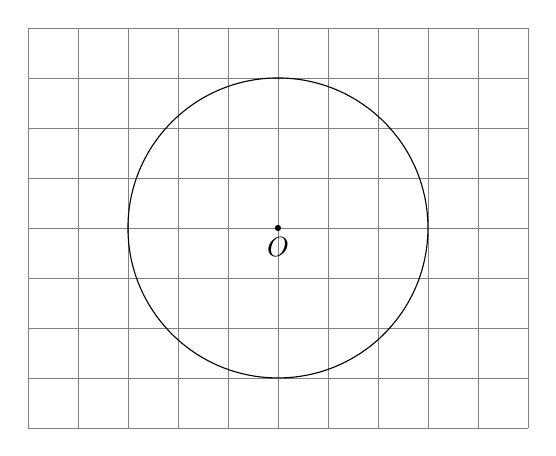
\begin{tikzpicture}[scale=.635]
      \draw [help lines] (-5,-4) grid (5,4);
      %\draw [thick, ->] (-2.2,0) -- (10.4,0) node [below right] {$x$};
      %\draw [thick, ->] (0,-2.2)--(0,10.4) node [left] {$y$};
      \draw (0,0) circle [radius=3] node[below]{$O$};
      \draw [fill] (0,0) circle [radius=0.05];
    \end{tikzpicture}
  \end{multicols}

    
\item Find the area of the shape shown below composed of a rectangle and circular cap. Leave your answer as an exact value in terms of $\pi$.
\begin{flushright}
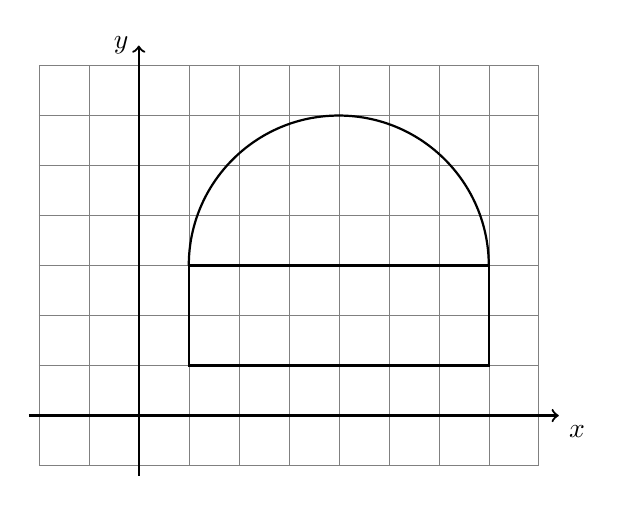
\begin{tikzpicture}[scale=.635]
  \draw [help lines] (-2,-1) grid (8,7);
  \draw [thick, ->] (-2.2,0) -- (8.4,0) node [below right] {$x$};
  \draw [thick, ->] (0,-1.2)--(0,7.4) node [left] {$y$};
  \draw [thick] (1,1)--(7,1)--(7,3)--(1,3)--cycle;
  %\draw [thick] (3,4) arc (90:270:1);
  \draw [thick] (7,3) arc (0:180:3);
\end{tikzpicture}
\end{flushright}

\newpage
\item Find the volume of a pyramid ($V=\frac{1}{3}Bh$) having a height of 11.3 inches and with a square base having side lengths of 7 inches. Express your result to the \emph{nearest cubic inch}. \vspace{3cm}

\item The side $\overline{AB}$ of triangle $ABC$ is extended and an altitude to the vertex $C$ is drawn, as shown below. The triangle's height is $h=7.25$ and its base measures $AB=12.4$. Find the area of the triangle.\\[0.25cm]
   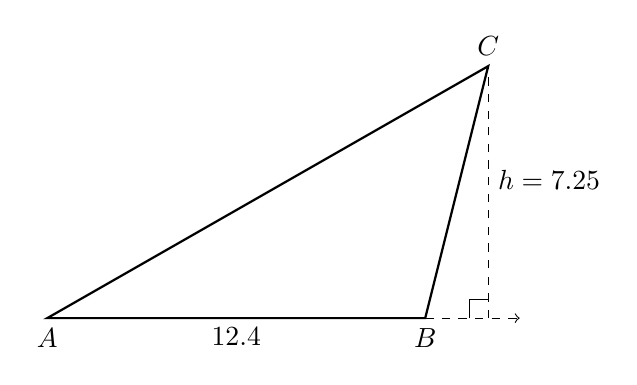
\begin{tikzpicture}[scale=0.8]
     \draw [thick]
       (0,0)node[below]{$A$}--
       (6,0)node[below]{$B$}--
       (7,4)node[above]{$C$} --cycle;
    \draw [dashed] (7,0)--(7,4);
    \draw [dashed, ->] (6,0)--(7.5,0);
    \draw (7,0)++(-0.3,0)--++(0,0.3)--+(0.3,0);
    \node at (7,2.2)[right]{$h=7.25$};
    \node at (3,0)[below]{$12.4$};
  \end{tikzpicture}

\item Find the volume of a sphere with a radius of 30 inches, to the \emph{nearest whole cubic inch}. (The formula for the volume of a \emph{sphere} is $V=\frac{4}{3}\pi r^3$) \vspace{3cm}

\item A rectangle has an area of 44 square inches. Its width is 4 inches. Find its length.
 \vspace{2.0cm}

\item A triangle has an area of 75 square centimeters. Its height is 12 centimeters. Find the length of its base.
\end{enumerate}
\end{document}